This section explains and motivates the method used for the experiment tested in this thesis. First, we provide a summary of the method used, as this will help to give the overall procedure without getting stuck in the details. Then, a detailed description of each different part will be given. 


\begin{generalinstructions}
    \begin{compactenum}
        \item Method overview
        \item Test of marginal model (does it deviate for some different distributions)
        \item Choice of method for copula
        \item Portfolio testing (Actual experiment)
    \end{compactenum}
\end{generalinstructions}


%%%%%%%%%%%%%%%%%%%%%%%%%%%%%%%%%%%%%%%%%%%%%%%%%%%%%%%%%%%%%%%%%%%%%%%%%%%%%%%
%%%% Method overview
%%%%%%%%%%%%%%%%%%%%%%%%%%%%%%%%%%%%%%%%%%%%%%%%%%%%%%%%%%%%%%%%%%%%%%%%%%%%%%%
\subsection{Method overview}
\todo{Connect to research question and hypothesis}
This section describes the method used for the experiment. The method is divided into three main parts. 

First, a test of the marginal model is performed to see how well the marginal distributions are fitted. This is to see if the marginal distribution fitted by the marginal model works as intended. Theoretically there should not be any difference between the fitted marginal distribution and the true distribution of the data  given a sufficient number of samples. This is important as the copula is invariant to strictly increasing transformations, meaning that the fitted copula should be able to replicate the joint distribution of the data regardless of the marginal distributions used. In the main experiment we will know that the log returns are normally distributed. In reality this is not always the case, and therefore we want to test how well the \gls{NC} marginals works.

The second part of the method is to test how the neural copula should be trained. This is done by testing different training schemes for the \gls{NC}. The goal of this part is to find a method that works universally for the neural copula meaning that the trained copula model produces a valid copula function that fits the data well. This is done by testing different training schemes and comparing the fitted copulas to one another. This is all to find a method that works well for the \gls{NC} meaning that the fitted copula is valid. 

The third part of the method is the main experiment of this thesis and the overall procedure is as follows. \todo{illustrate workflow} To begin with, different portfolios with different types of dependency structures will be generated. This will be done by sampling data in probability space from different copulas and transforming it to return space using the \gls{ITM} to obtain dependent normally distributed returns, as described in \Cref{sec:CopulaUseCase}. This ensures that the marginal distributions of the created portfolios have normal marginal distributions, removing the need for fitting them in this experiment. This allows for an evaluation of the pure performance of the copula, without conflating it with potential errors from fitting marginal distributions. The generated normally distributed random numbers are then used as the random shocks from the Weiner process when simulating the \gls{GBM} using the Euler-Maruyama scheme to replicate stock price time series. This creates a realistic setting for when using copulas would be suitable.  

The generated price time series are then divided into two different parts. These different parts represent the historical and the future returns of the portfolios. The splitting of data is illustrated in \Cref{fig:DataDivision} where the blue and orange lines are different simulated stocks over time. The price time series are divided to create the fit and test parts. The historical part is used for fitting the different copulas, while the future part can be considered the true distribution of future returns. As described when introducing \gls{MC} methods in \Cref{sec:MonteCarlo}, the key assumption is that of the statistical distribution of the data and that the distribution remains the same in the future. Hence the historical data is used to fit the copulas to the historical data. From the fitted copula random numbers replicating the joint distribution is generated. If the copula adequately captures the dependence the generated data from the fitted copula should be similar to the future data. This is the main goal of this thesis, to evaluate how well different copulas can replicate the joint distribution of the data. An example of the what the different distributions can look like for the test data compared to the data sampled from the fitted copula can be viewed in \Cref{fig:TestSampleComparison} where the red data is the testing data from a Clayton copula that is to be replicated and the blue data is the data sampled from the fitted gaussian copula. If the copula performs well when fitted, these datasets should be similar. 

\begin{figure}
    \centering
    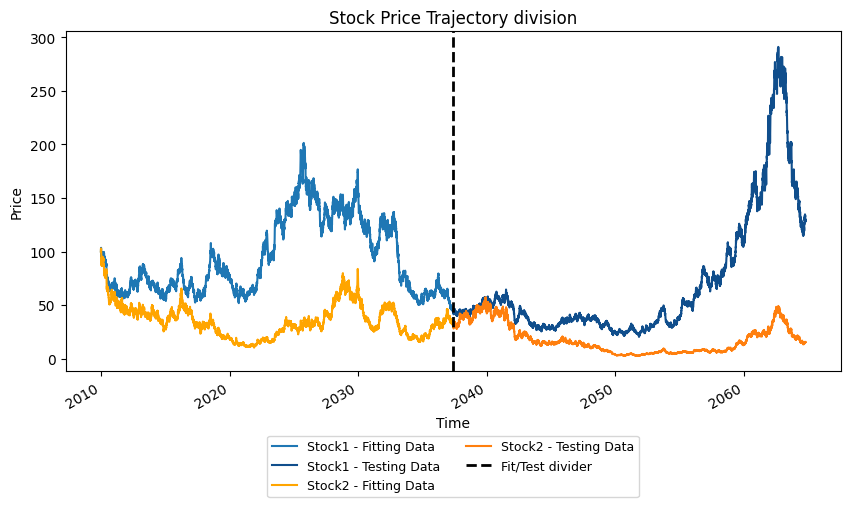
\includegraphics[width=0.8\textwidth]{4Method/pictures/DataDivision.png}
    \caption{Illustration of how the data is divided into fitting and testing parts. }
    \label{fig:DataDivision}
\end{figure}

\begin{figure}
    \centering
    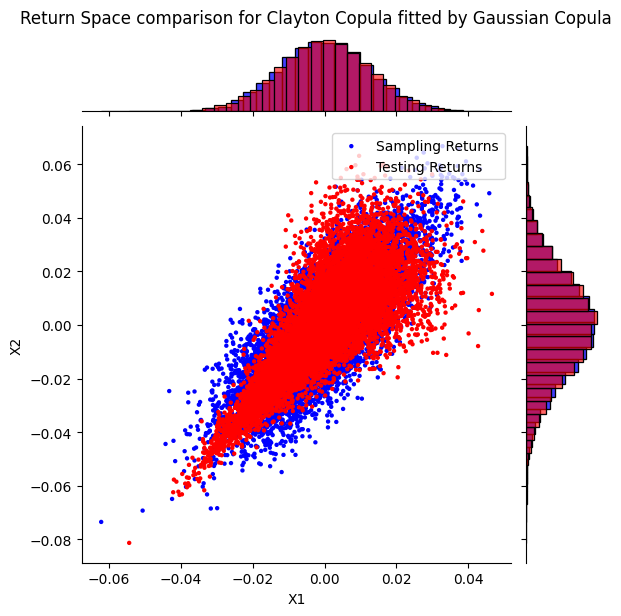
\includegraphics[width=0.5\textwidth]{4Method/pictures/TestSampleComparison.png}
    \caption{Figure illustrating the difference between the test data and the data sampled from the fitted copula. }
    \label{fig:TestSampleComparison}
\end{figure}

To evaluate the various copulas' ability to accurately capture the dependence between random variables, it is therefore sensible to compare the generated data to the testing data. The reason for using simulated data in this experiment is to ensure that the joint distribution is constant over time as this is a key assumption when using \gls{MC} methods. If the data generated from the fitted copula is similar to the testing data, it shows that the dependence is appropriately modeled by the copula. If not, it shows that the copula is not well suited to model the dependence. Hence this is a good way to evaluate the copulas' performance in an isolated manner. 

To emphasize the key assumption when using copulas to simulate data for Monte Carlo purposes. The assumption is that the joint distribution observed in the past continues to be the distribution from which the data is generated into the future. 

To quantify how similar the test and sampled datasets are to each other, the distance measure described in \Cref{sec:GoodnessOfFit} is used. This allows for computing an average distance that each copula is from the test data over several datasets. This makes it possible to evaluate which copula performs best overall.  


%%%%%%%%%%%%%%%%%%%%%%%%%%%%%%%%%%%%%%%%%%%%%%%%%%%%%%%%%%%%%%%%%%%%%%%%%%%%%
%%%% Marginal model test
%%%%%%%%%%%%%%%%%%%%%%%%%%%%%%%%%%%%%%%%%%%%%%%%%%%%%%%%%%%%%%%%%%%%%%%%%%%%%
\subsection{Marginal model test}
To validate that the marginal model works as intended, a test is performed to see how well the fitted marginal distribution matches the true distribution of the data. This is done by generating data from a known distribution and then fitting a marginal model to it. The fitted marginal model is then compared to the true distribution of the data by transforming the data to probability space using the \gls{PIT} using both the fitted distribution and the true distribution. To evaluate how similar the points in probability space are to each other the \gls{MAE} is calculated. Additionally a QQ-plot is created to visualize how well the fitted distribution matches how well the data follows the true distribution. During this experiment it is important to keep in mind that the generated data is subject to random noise, therefore it is not necessarily the case that the true distribution is the same as the observed distribution even tough they should be the same. It is however a good benchmark to see how well the fitted distribution matches the true distribution, which would be a reasonable choice of distribution to use if the neural network was not used. The distributions used for the test are listed in \Cref{tab:distributions} where the distribution, the parameter values, and a short description is displayed for each of the tested distributions.


\begin{table}[h]
    \centering
    \caption{Distributions and parameters used for the marginal model test.}
    \begin{tabular}{@{}ccl@{}}
        Distribution & Parameters & Description \\
        \toprule
        Gaussian & $\mu=0, \sigma=1$ & Standard normal distribution \\ 
        Student's $t$ & $\nu=5$ & Student's t-distribution with 5 degrees of freedom \\ 
        Uniform & $a=0, b=1$ & Uniform distribution on [0, 1] \\ 
        Exponential & $\lambda=1$ & Exponential distribution with rate 1 \\ 
        Laplace & $\mu=0, b=1$ & Laplace distribution with mean 0 and scale 1 \\ 
        Log-normal & $\mu=0, \sigma^2=1$ & Log-normal distribution with mean 0 and variance 1 \\ 
    \end{tabular}
    \label{tab:distributions}
\end{table}



%%%%%%%%%%%%%%%%%%%%%%%%%%%%%%%%%%%%%%%%%%%%%%%%%%%%%%%%%%%%%%%%%%%%%%%%%%%%%
%%%% Neural copula testing 
%%%%%%%%%%%%%%%%%%%%%%%%%%%%%%%%%%%%%%%%%%%%%%%%%%%%%%%%%%%%%%%%%%%%%%%%%%%%%
\subsection{Neural Copula training scheme test}
In this section the procedure for finding a method that reliably obtains valid copula functions in training. Wether or not a copula function is valid is determined by wether or not it satisfies the conditions of being a copula defined in \Cref{def:copula}. In practice for the neural copula this means that all but the first of the loss terms, defined in \Cref{sec:NeuralCopulaLoss}, should approach zero when training is done. Several different training schemes will be tested with the goal of finding a method that works well for the neural copula meaning that the fitted copula is valid.

Several datasets will be used for testing the neural copula fitting procedure. This is to ensure that the method works well, regardless of the data, consistently resulting in valid copulas. The method for this workflow is as follows for each dataset. First different datasets will be generated \todo{How} and a grid of different parameter values will be created. The grid will contain different values for the parameters of the neural copula such as the solver used, learning rates, number of epochs, batch size, network architecture, number of data points in the additional uniform datasets. This creates a large number of different combinations of choices to test which will hopefully result in a method for finding a training method that works well universally.  

The datasets that will be used for testing the neural copula fitting procedure are:\\ 
Independence copula Gaussian with 0 correlation\\
Gaussian with +/-0.7 correlation\\
Frechet-Hoeffding upper bound\\
Frechet-Hoeffding lower bound\\




For each of the combinations in the grid the an ensemble of runs will be performed to mitigate the impact of what random seeds are used for initializing the weights of the network. The ensemble will consist of 10 runs for each combination in the grid. The best run from the ensemble will be kept for each combination in the grid. 

For each of the different runs in the ensemble both a several different schemes for training the neural copula will be tested. The first scheme is to train the copula on the dataset without any pretraining. The second scheme is to pretrain the copula on a dataset generated from the independence copula and then using the weights of the pretrained copula to initialize the weights of the neural copula when training on the dataset. There are three different variations of this pretraining scheme. The first is to train the copula on the independence copula using the full loss function defined in \Cref{sec:NeuralCopulaLoss}. The second is to train the copula on the independence copula using the loss function without the L1 term. The third is to train the copula on the independence copula using only the MSE as loss function. The rationale behind pretraining this is that this should produce a network mimicking the independence copula which can be thought of as a middle ground between the upper and lower Frechet-Hoeffding bounds. This is potentially a good starting point for the weights when fitting the copula to other data.  

After pretraining, the neural copula is trained on the dataset using the weights from pretraining as a starting point. The starting weights in each of the pretraining schemes are saved so that after evaluation they can be used as a starting point for training the copula on a dataset. This will be needed in the final experiment of this thesis, described in \Cref{sec:PortfolioTesting}, where the best training scheme and initial weights will be used for the \gls{NC}. 

After training the best overall method over each of the datasets will be used evaluated by validating that the losses relating to the copula function constraints are almost zero. This indicates that the fitted copula is valid. Of the methods that do not violate the copula definition the method that has the best fit overall will be declared the best one and hence be used in the final experiment, described in \Cref{sec:PortfolioTesting}.  

\begin{generalinstructions}
Given generated datasets and a specified grid\\
\textbf{For each dataset}
\begin{compactitem}
    \item Fit marginal models
    \item \textbf{For grid alternative}
    \begin{compactitem}
        \item \textbf{For run in ensemble}
        \begin{compactitem}
            \item \textbf{Normal Training save weights} 
            \begin{compactitem}
                \item Train copula on dataset
            \end{compactitem}
            \item \textbf{Using Pretraining}\\
            \textbf{Pretraining on independence copula save weights}
            \begin{compactitem}             
                \item Full loss function
                \item Training without L1 term in loss function
                \item Training with MSE loss function
            \end{compactitem}
            \textbf{Posttraining on dataset starting at pretraining end weights}
            \begin{compactitem}             
                \item Training on dataset for each pretraining scheme
            \end{compactitem}
        \end{compactitem}
        \item \textbf{Choose best run in ensemble keep weights for that run (to use if the method is used)}
    \end{compactitem}
\end{compactitem}
\textbf{Evaluate the average performance of methods over the datasets}
\end{generalinstructions}



Neural copula what ive tested (state best and tell what ive tested)

 
\todo{How have i changed the neural copula approach, errors in the neural copula article.}


%%%%%%%%%%%%%%%%%%%%%%%%%%%%%%%%%%%%%%%%%%%%%%%%%%%%%%%%%%%%%%%%%%%%%%%%%%%%%%
%%%% Portfolio testing
%%%%%%%%%%%%%%%%%%%%%%%%%%%%%%%%%%%%%%%%%%%%%%%%%%%%%%%%%%%%%%%%%%%%%%%%%%%%%%
\subsection{Portfolio testing}\label{sec:PortfolioTesting}
This section details the steps in the test of the copulas on the different portfolios. 

\subsubsection{Data Generation}
To evaluate the performance of different copulas when fitting them to data. Given that this thesis focuses on the use of copulas for modeling financial returns, we want to create test portfolios consisting of pairs of stocks. These portfolios should ideally cover a wide range of dependence structures to test the different copulas' versatility and robustness in varying conditions. 

This thesis focuses on the role of the copula purely and therefore, the aim is not to conflate the results from the copula's performance with that of the marginal fitting procedure. Therefore, we want each marginal distribution of the generated portfolios to be the same known distribution. The marginal distributions used should not matter, given that the copula is invariant to strictly increasing transformations as stated in \Cref{the:TranslationInvariance}. In this study, it is advantageous to remove the need for fitting the different marginal distributions, by just using the normal distribution. If having different marginal distributions the number of combinations to test during model fitting becomes large.  \todo{Add reference saying that marginal dist fitting is studied.}

To generate portfolios with different dependence structures and the same marginal distributions, copulas will be used. This will be done by first sampling data from analytical copulas with different parameter values. This will result in data points in probability space that contain the pure dependence between the different variables. These data points will then be plugged into the inverse \gls{CDF} of a Standard normal distribution. This performs the \gls{PIT} in reverse, creating data points with standard normal marginal distributions with the dependence described by the copula. 

After having generated these pairs of dependent standard, normally distributed random numbers, they are used as the random shocks when simulating the bivariate \gls{GBM} using the Euler-Maruyama scheme.\todo{as defined in...} This results in the test portfolios replicating stock prices over time, creating a realistic setting for when using copulas is appropriate. 

The above procedure is used with the following copulas and parameter values. 
\todo{Decide on portfolios, and time horizon, and mean and volatility}

The data generated is divided into a fitting and a testing part. The fitting part will be used in the model fitting and can be thought of as historically observed data. The testing part will be used in the model evaluation and can be thought of as data that will appear in the future, which we want to replicate as well as possible by fitting a copula to the historical data. 

\subsubsection{Model Fitting}
The fitting data from each of the previously generated portfolios is used for fitting the different copulas. To do this, the data needs to be converted so that the copulas can work with it. Hence, the log returns are calculated as defined in \Cref{def:logReturns}. These are then standardized and centered to have a zero mean and unit variance. \todo{maybe not necessary to scale...}

The different types of copulas are then fitted as described for the Gaussian in \Cref{sec:GaussianCopula}, the Student's $t$ in \Cref{sec:StudentsCopula}, the Clayton in \Cref{sec:ClaytonCopula} and the \gls{NC} in \Cref{sec:NeuralCopulaFittingAndSampling}. 


\subsubsection{Model Sampling}
The main use for copulas is arguably to sample random numbers to be used in \gls{MC} simulations \Citet[p.~40]{Nelsen2006}. The random numbers from the copula can be used to generate dependent realizations of a pair of random variables, regardless of their marginal distributions. Hence, it should make sense to evaluate the copulas based on how well generated random numbers from a fitted copula replicates the true dependence structure of the data. The procedures for sampling from the copulas is described for the Gaussian in \Cref{sec:GaussianCopula}, the Student's $t$ in \Cref{sec:StudentsCopula}, the Clayton in \Cref{sec:ClaytonCopula} and the \gls{NC} in \Cref{sec:NeuralCopulaFittingAndSampling}. 

The sampled data points from the copulas, other than the \gls{NC} which uses the inverse marginal models, are inserted into the inverse normal distribution and then scaled to match the observed standard deviation of the fitting data. This should generate data similar to the data in the testing part if the copula adequately captures the dependence in the data.

\subsubsection{Model evaluation}
To evaluate the performance of each copula for each of the datasets the distance measure described in \Cref{sec:GoodnessOfFit} is used. An average of the distance measure is calculated over the different datasets for each copula. This will give a good indication of how well each copula performs overall. 


\begin{generalinstructions}
    \begin{compactenum}
        \item Data generation
        \begin{compactenum}
            \item Generate returns
            \item Put into GBM as random shocks 
            \item Calculate log returns 
            \item Split into different parts (train - test)
            \item Normalize and center data
        \end{compactenum}
        \item Model fitting (for each copula)
        \begin{compactenum}
            \item Fit marginal on training data if necessary (only for neural) 
            \item Perform PIT on training
            \item Fit copula functions on transformed training
        \end{compactenum}
        \item Model evaluation
        
        \textbf{Alternative 1}
        \begin{compactenum}
            \item Sample new returns based on fitted model
            \item Compare on distribution level to the testing data
        \end{compactenum}
        \textbf{Alternative 2}
        \begin{compactenum}
            \item Compare fitted copula to empirical copula of test data
        \end{compactenum}
    \end{compactenum}
\end{generalinstructions}

